\chapter{Results}
\label{chap:results}

In this chapter we will present the results of applying the methods discussed previously to the data in the blockchain and data we have gathered from the LN. Bitcoin has a testnet used for development and experimental functionality in which the LN have been tested for longer than it has been used on the mainnet. We have used both the testnet and the mainnet in our project; our reasoning for this is the LN on the testnet is bigger, and people are testing a wide array of use cases and functionality using testnet coin without any value; while on the mainnet users have to use Bitcoin with value, but this can result in more realistic user behaviour which impacts the data generated.
By using both Bitcoin networks we will have one with more edge cases and more data, and one containing data reflecting real user behaviour.
The testnet has its own blockchain as the mainnet and is therefore publicly available in the same manner. Collecting data from the LN as we discussed in \cref{sec:ln_analysis} was done in two intervals of one week each. Creating a snapshot of the network on each block for a week results in about 1000 blocks worth of data. This should be sufficient to verify our methods of identifying relevant LN transactions, but doing this twice also allowed us to make adjustments after the results of the first interval.

\section{Method verification with LN data}

Comparing data from the LN with our data from the blockchain provided us with results about the extent our identification methods was able to locate LN channels on the blockchain and to which degree. There is three sets with data was used in these comparisons: 
\begin{itemize}
    \item The set \( \alpha \) , counting channels from the LN closed during the capture interval. 
    \item The set \( \beta \), containing channels from the blockchain identified using timelocked redeem scripts,
    \item The set  \( \gamma \), containing potential channels identified on the blockchain using 2of2 multisig scripts.
\end{itemize}

As we stated in \cref{sec:bc_analysis} and \cref{subsec:pcln} a LN channel uses the P2WSH 2of2 multisig type for the on chain founding - closing output - input pair, and we discussed how this could be used to give us a set of potential transactions being related to LN channels by discarding other types of transactions. Because the on-chain channel transactions must be of this type the \( \gamma \) set is guaranteed to include all channels closed in the block interval used for the search. It also means that the two other sets will be subset of \( \gamma \). So the relations between the sets should be as follows:

\begin{equation} \label{eq:1}
      \alpha \subseteq \gamma, \hspace{10pt} \beta \subseteq \gamma, \hspace{10pt} \beta \subseteq \alpha  
\end{equation}

The two first relations is explained above and is always true for the systems in its current case. The last relation however, will not hold with our data, but ideally it should be true. For this to be the case our method with timelocked redeem scripts for identifying channels should not have any false positives-i.e., identify channels which is unrelated to the LN. We should also be able to discover all closed channels from the LN during the interval, so we get the complete set of actual channels-i.e., \( \gamma \) contain all LN channels closed in the interval. While the timelocked scripts are very unique and therefore good for identifying channels, and theoretically one could synchronize and get all LN channels through the network, this would only always be true in a ideal world scenario. So as we will see with our data \( \beta \not\subseteq \alpha \), but keeping the relation in mind will be useful when analyzing the data.

\subsection{First Interval}

\begin{figure}[h]
    \centering
    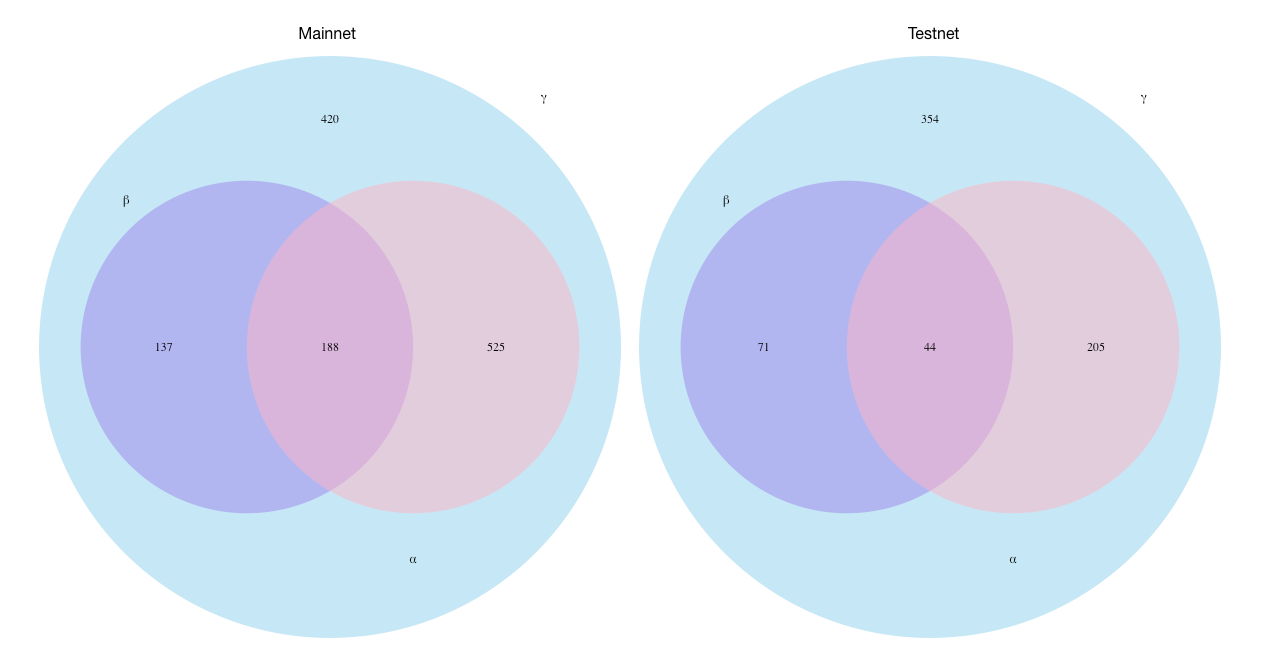
\includegraphics[width=16cm]{figures/graphs/venn_full1.png}
    \caption{Venn diagram of channel sets in interval one}
    \label{fig:venn_run1}
\end{figure}

The first interval for the mainnet had a length of 1151 blocks between block 517855 and 519005. Our modified LND implementation described in \cref{chap:metodology} collected data from the LN and produced the set \( \alpha \) containing 713 channels which where closed during this interval. The same interval on the blockchain was parsed two times, once identifying channels using timelocked redeem scripts, and a second time getting all potential channels using multisig identification. This resulted in a \( \beta \) set containing 325 channels and a \( \gamma \) set with 1270 channels shown on the left left in \cref{fig:venn_run1} as a venn diagram. We can see how both \( \beta \) and \(\alpha\) is a subset of \( \gamma\), but \(\beta \not\subseteq \alpha\). The intersection \(\beta \cap \alpha\) is the number of channels we identified using the timelocked method which was also found trough the LN node. On the mainnet this intersection was 188 which is 26.37\% of total channels in \( \alpha \). This is reasonable as the method will only discover a channel if it has been unilaterally closed as we explained in \cref{sec:bc_analysis} and not if a channel is closed cooperatively which likely will happen more frequently. We should also note the large \( \beta \backslash{} \alpha \) relative compliment of \( \alpha in \beta \) is 137 which is 42.15\% of of the channels in \(\beta\). Having a false positive this high is very unlikely because the uniqueness of the timelocking redeem scripts, so we made the assumption that these are actually LN channels which we have not been able to capture in our interaction with the LN. \todo{add for interval 2 more peers}
This means we can assume the union \(\alpha \cup \beta \) are all LN channels, which would mean the total number of LN channels closed in this interval is 1038. The potential multisig 




\subsection{Second Interval}


\begin{figure}[h]
    \centering
    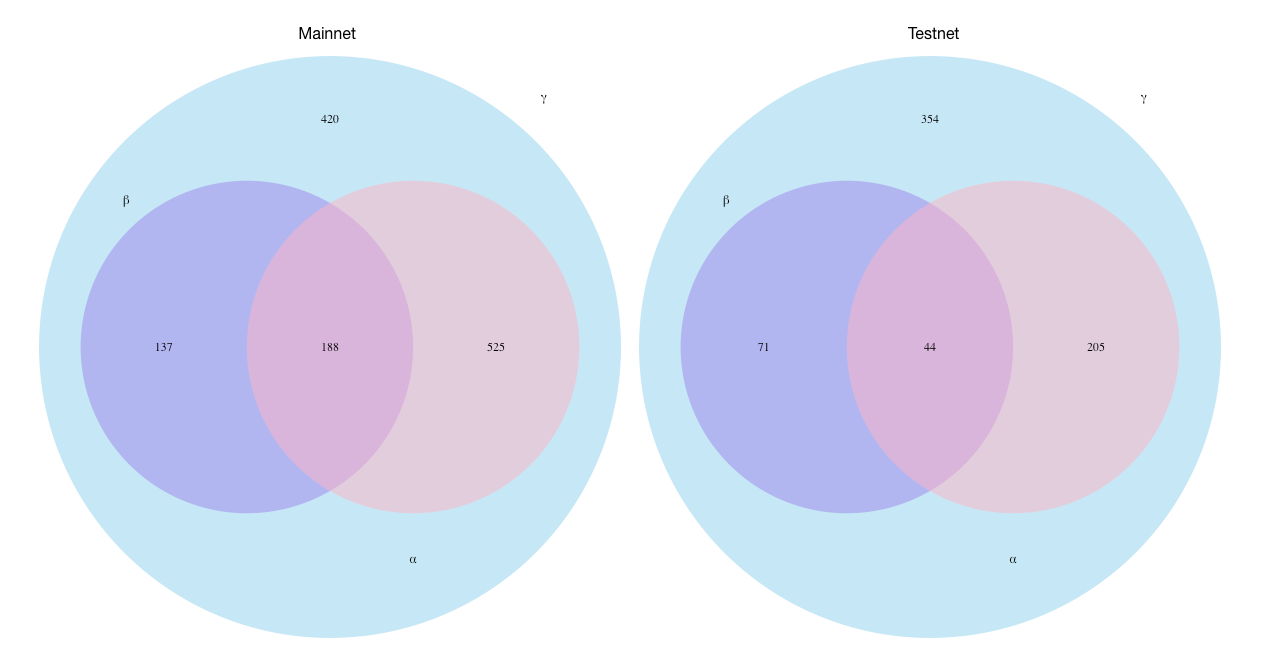
\includegraphics[width=16cm]{figures/graphs/venn_full1.png}
    \caption{Venn diagram of channel sets in interval one}
    \label{fig:venn_run2}
\end{figure}



\section{LN size}

\begin{figure}[h]
    \centering
    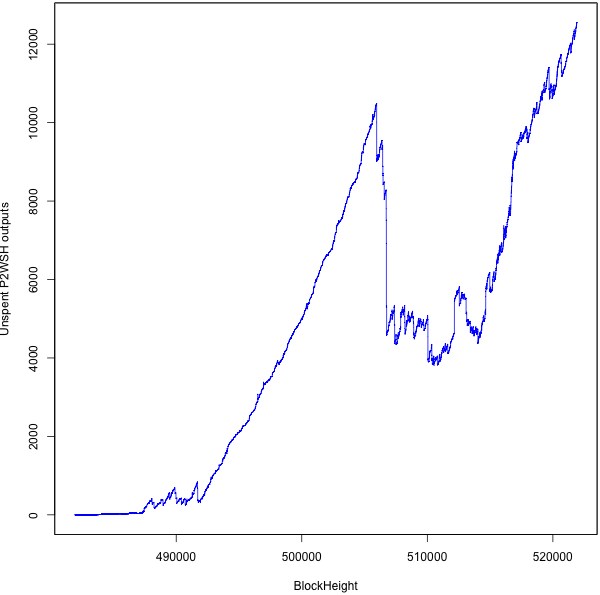
\includegraphics[width=10cm]{figures/graphs/lnsize_mainnet.png}
    \caption{Maximum size of the LN based on unspent P2WSH outputs on the blockchain}
    \label{fig:htlc_bc}
\end{figure}

\begin{figure}[t]
    \centering
    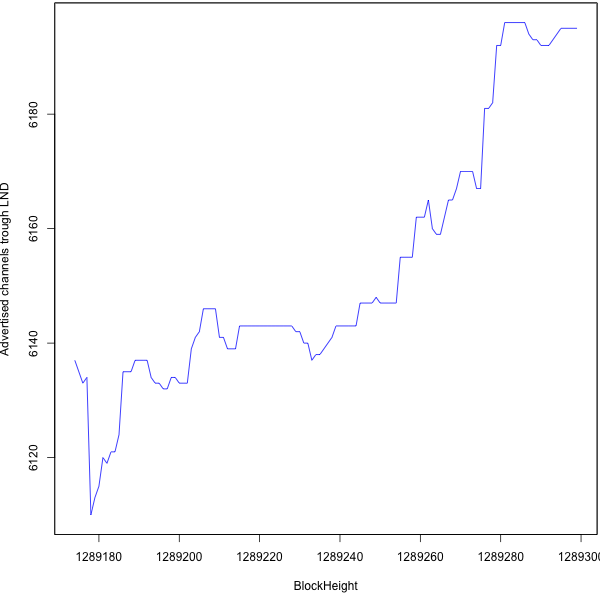
\includegraphics[width=10cm]{figures/lnsizeTS.png}
    \caption{Channel count from LN on testnet}
    \label{fig:htlc_bc}
\end{figure}


\section{Other metrics}

% single founded vs multiple founded txs.
% channel size
% channel lifetime

\section{Clustering}

\begin{figure}[h]
    \centering
    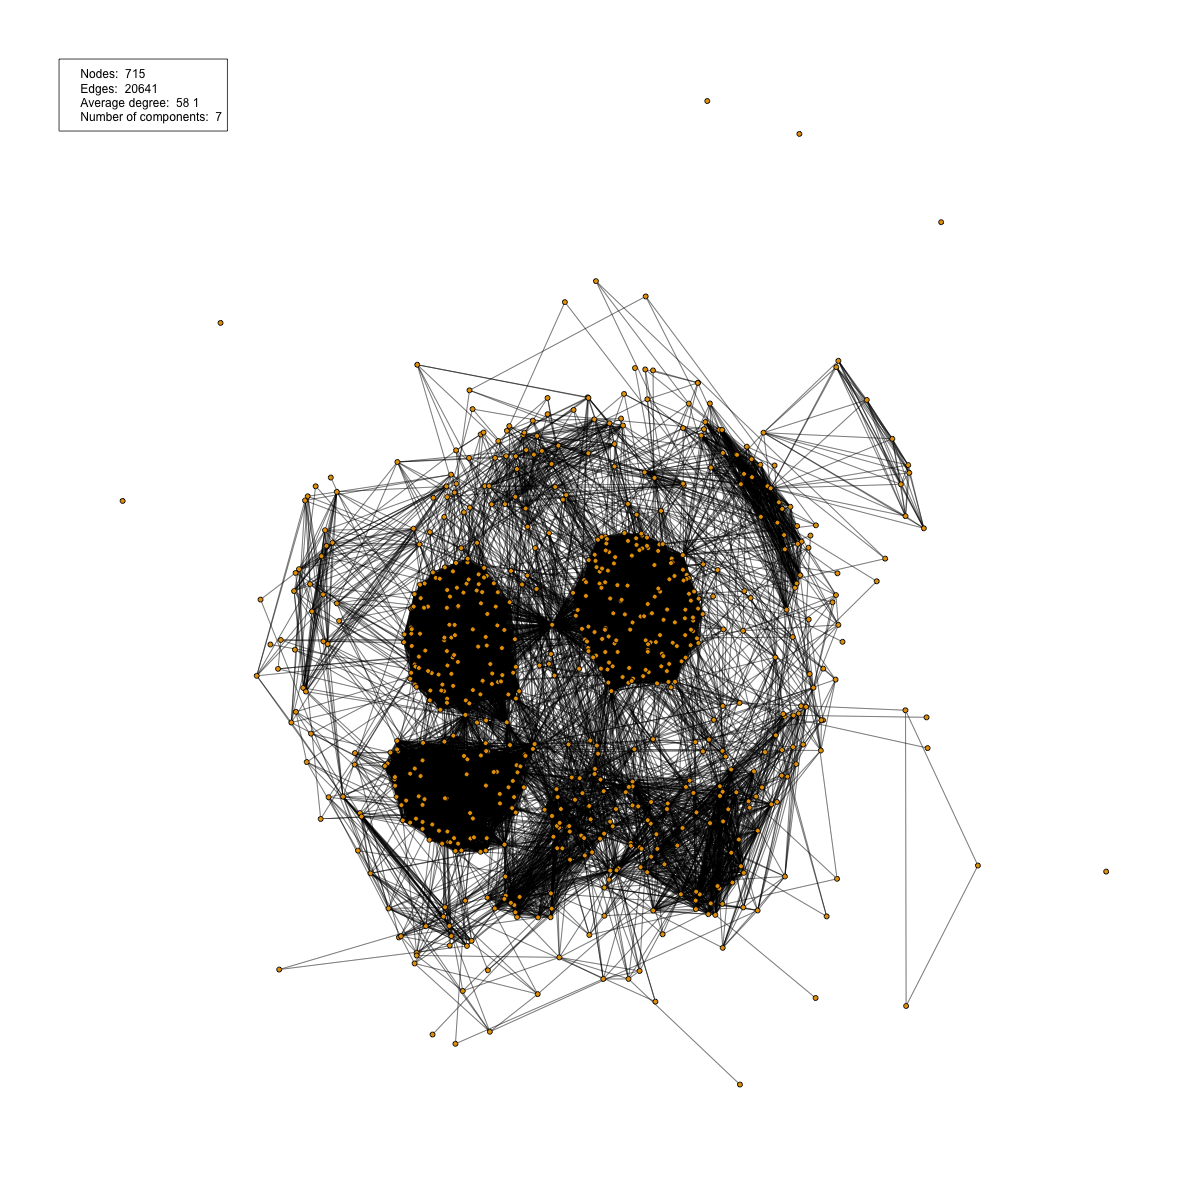
\includegraphics[width=14cm]{figures/graphs/cg_ln_mainnet_run1.png}
    \caption{Linked channels from LN mainnet run1}
    \label{fig:channelGraphLNTS}
\end{figure}

\begin{figure}[h]
    \centering
    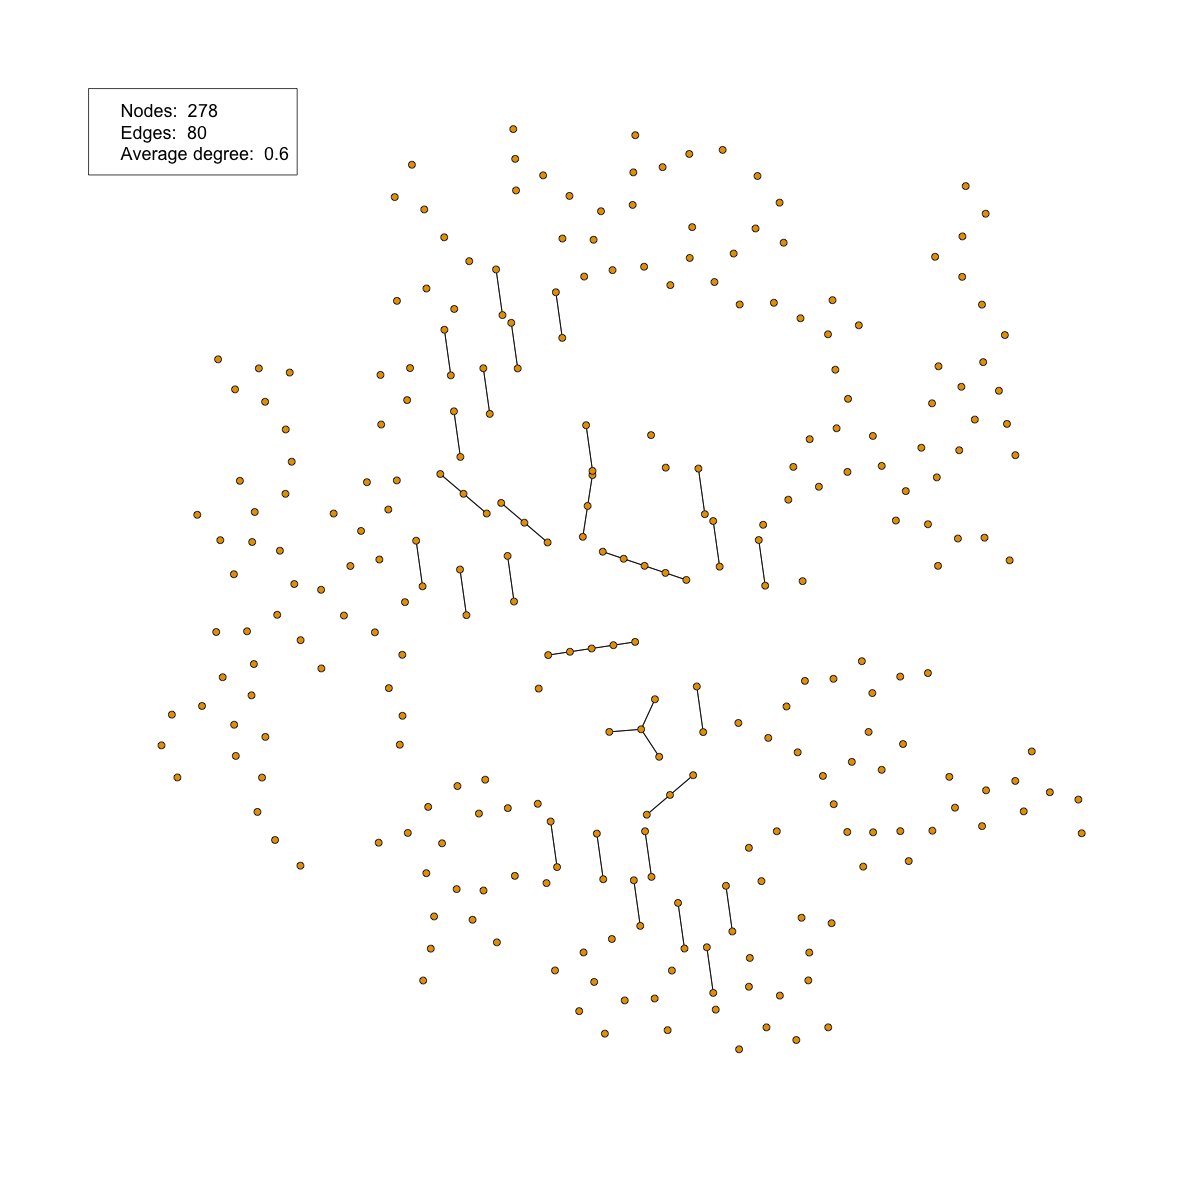
\includegraphics[width=14cm]{figures/graphs/cg_bc_mainnet_run1.png}
    \caption{Linked channels from BC mainnet run1}
    \label{fig:channelGraphLNTS}
\end{figure}